To uncover the elusive extent repair bug in \Azure Storage vNext, its developers wrote a test harness using \psharp. The developers expected that it was more likely for the bug to occur in the ExtMgr logic, rather than in the EN logic. Hence, they focused on testing the real ExtMgr using modeled ENs. The test harness for vNext consists of the following \psharp machines (as shown in Figure~\ref{fig:azurestoremodel}):
\begin{description}
\item[ExtentManager] acts as a thin wrapper machine for the real ExtMgr component in vNext (see \S\ref{sec:method:wrap_target}).

\item[ExtentNode] is a simple model of an EN (see \S\ref{sec:method:mock_en}).

\item[Timer] exploits the nondeterministic choice generation available in \psharp to model timeouts (see \S\ref{sec:method:timer}).

\item[TestingDriver] is responsible for driving testing scenarios, relaying messages between machines, and injecting failures (see \S\ref{sec:method:driver}).

\item[RepairMonitor] collects EN-related state to check if the desired liveness property is satisfied (see \S\ref{sec:method:monitor}).
\end{description}

\begin{figure}[t]
\centering
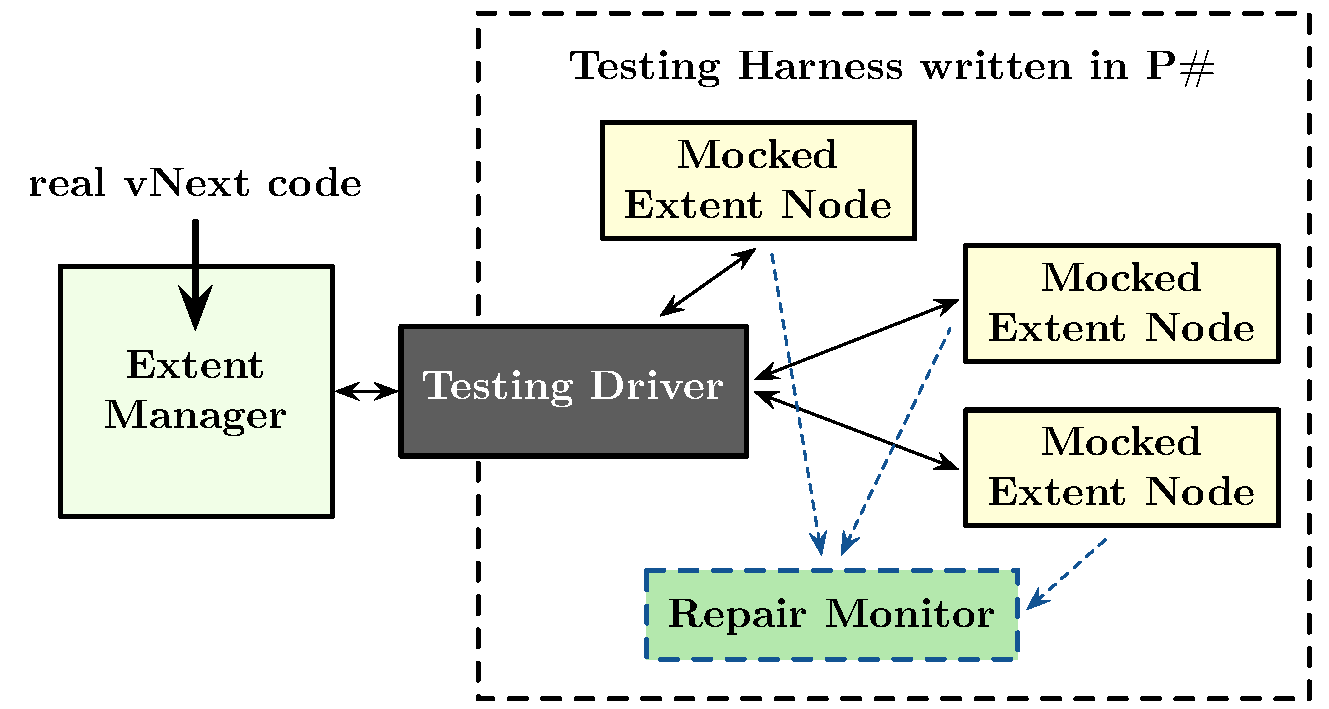
\includegraphics[width=\linewidth]{img/mocked_vnext}
\caption{Real Extent Manager with a modeled environment (each box represents one \psharp machine).}
\label{fig:azurestoremodel}
\vspace{-2mm}
\end{figure}

\subsection{The ExtentManager machine}
\label{sec:method:wrap_target}

\begin{figure}[t]
\begin{lstlisting}
// wrapping the target vNext component in a P# machine
class ExtentManagerMachine : Machine {
  private ExtentManager ExtMgr; // real vNext code

  void Init() {
    ExtMgr = new ExtentManager();
    ExtMgr.NetEngine = new MockedNetEngine(); // mock network
    ExtMgr.IsMockingTimer = true;	 // disable internal timer
  }

  [OnEvent(ExtentNodeMessageEvent, DeliverMessage)]
  void DeliverMessage(ExtentNodeMessage msg) {
    // relay messages from Extent Node to Extent Manager
    ExtMgr.ProcessMessage(msg);
  }
	
  [OnEvent(TimerTickEvent, ProcessExtentRepair)]
  void ProcessExtentRepair() {
    // extent repair loop driven by external timer
    ExtMgr.ProcessEvent(new ExtentRepairEvent());
  }
}
\end{lstlisting}
\vspace{-3mm}
\caption{The real Extent Manager is wrapped inside the \texttt{ExtentManager} \psharp machine.}
\label{fig:wrap_target}
%\vspace{-2mm}
\end{figure}

The real ExtMgr in vNext, which is our system-under-test, is wrapped inside the \texttt{ExtentManager} machine, as illustrated in the code snippet of Figure~\ref{fig:wrap_target}.

\begin{figure*}[t]
\centering
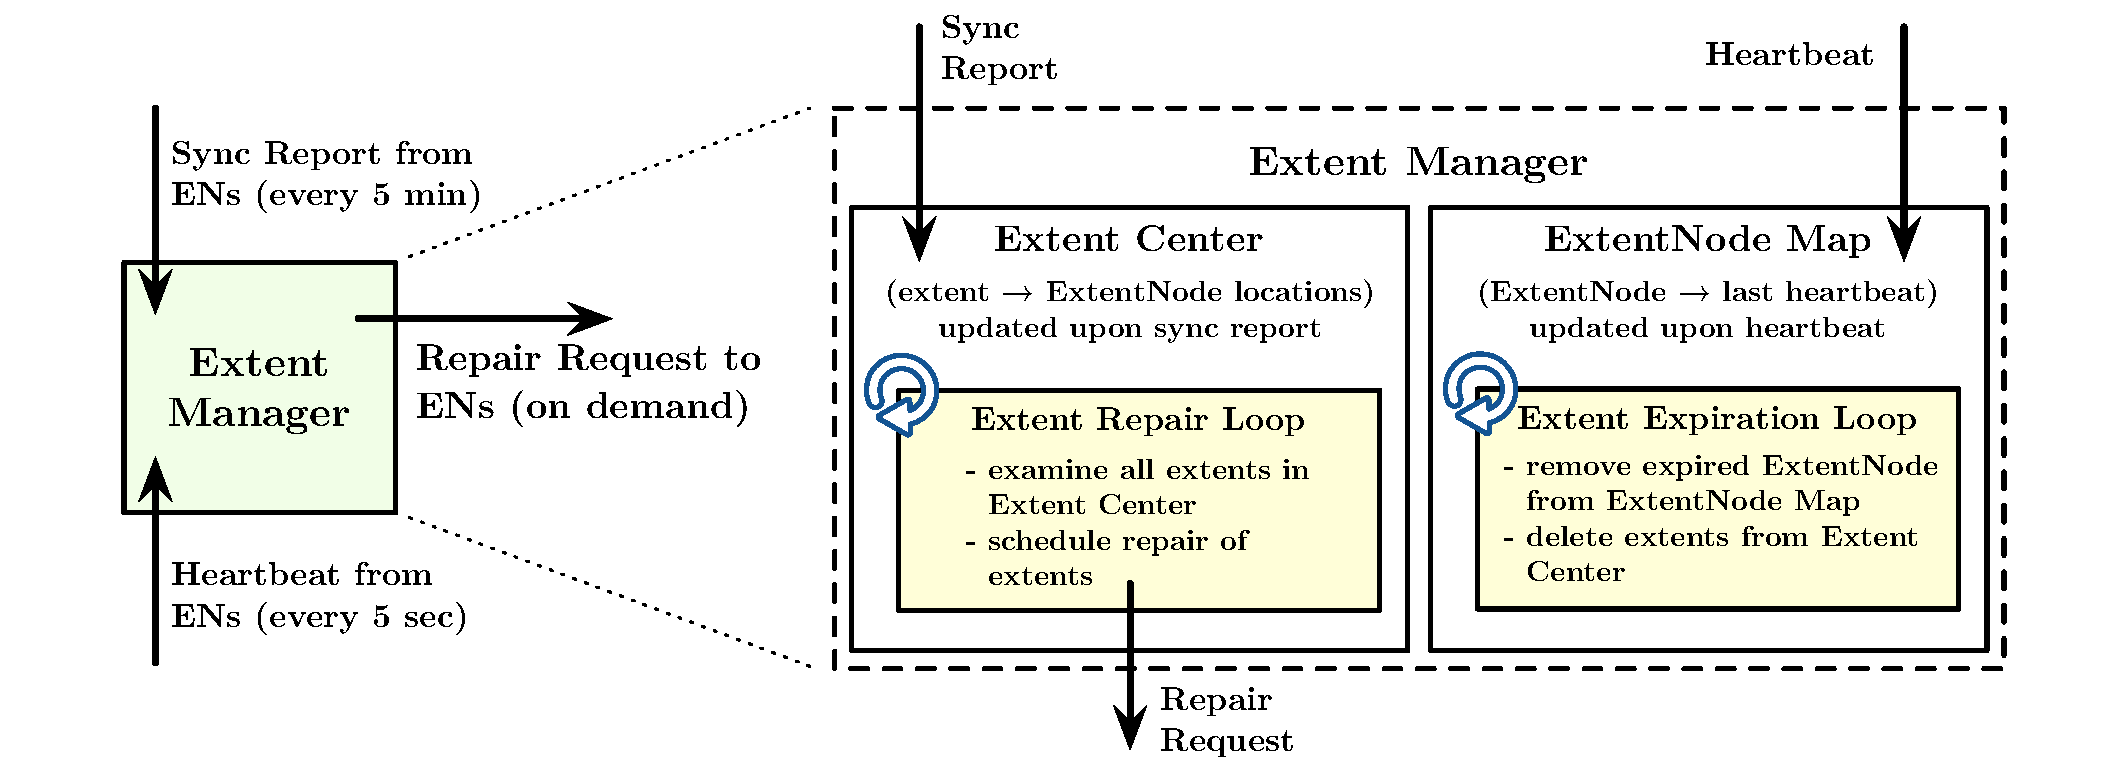
\includegraphics[width=.9\linewidth]{img/extent_manager}
\caption{Internal components of the real Extent Manager in \Azure Storage vNext.}
\label{fig:extentmanager}
\vspace{-5mm}
\end{figure*}

\textbf{Internals of the real Extent Manager}.
The real ExtMgr (see Figure~\ref{fig:extentmanager}) contains two data structures related to extent replication and repair: \texttt{ExtentCenter} and \texttt{ExtentNodeMap}. The \texttt{ExtentCenter} data structure maintains the records that map from extents to their hosting ENs. It is updated upon receiving the periodic sync reports from the ENs. Recall that the sync report from a particular EN lists all the extents stored at the EN. Its purpose is to update ExtMgr's possible out-of-date view of the EN with the ground truth. \texttt{ExtentNodeMap} records the latest heartbeat time from every EN.

ExtMgr internally runs a periodic \emph{EN expiration loop} that is responsible for removing ENs that have been missing heartbeats for an extended period of time, as well as cleaning up the corresponding extent records in \texttt{ExtentCenter}. In addition, ExtMgr runs a periodic \emph{extent repair loop} that examines all the \texttt{ExtentCenter} records, identifies extents with missing replicas, schedules extent repair tasks and sends them to the ENs.

\textbf{Intercepting network messages}.
The real ExtMgr uses a network engine to asynchronously send messages to the ENs. The \psharp test harness mocks the original network engine in vNext by overriding its interface. This enables the mocked network engine (we use the terms \textit{mocked} and \textit{modeled} interchangeably) to intercept all outbound messages and relay them to the \texttt{TestingDriver} machine, which is responsible for dispatching the messages to the corresponding \texttt{ExtentNode} machines. As shown in Figure~\ref{fig:enginecode}, the mocked network engine intercepts the outbound messages from the ExtMgr and invokes \texttt{PSharp.Send(...)} to asynchronously relay the messages to \texttt{TestingDriver}. This mocked network engine replaces the real network engine in the wrapped ExtMgr, as shown in Figure~\ref{fig:wrap_target}.

\begin{figure}[t]
\begin{lstlisting}
// network interface in vNext
class NetworkEngine {
  public virtual void SendMessage(Socket s, Message msg);
}

// mocked engine for intercepting Extent Manager messages
class MockedNetEngine : NetworkEngine {
  public override void SendMessage(Socket s, Message msg) {
    // intercept and relay Extent Manager messages
    PSharp.Send(TestingDriver, new ExtMgrMsgEvent(), s, msg);
  }
}
\end{lstlisting}
\vspace{-4mm}
\caption{Mocked network engine in vNext.}
\label{fig:enginecode}
\vspace{-2mm}
\end{figure}

Intercepting all network messages and dispatching them through the \psharp runtime is important for two reasons. First, it allows \psharp to systematically explore the interleavings between asynchronous event handlers in the system. Second, the mocked network engine could leverage the support for controlled nondeterministic choices in \psharp, and choose to drop the messages in a non-deterministic fashion, in case emulating message loss is desirable (not shown in this example).

Messages coming from the \texttt{ExtentNode} machines do \emph{not} go through the mocked network engine. They are delivered to the \texttt{ExtentManager} machine directly and trigger an action that invokes the messages on the wrapped ExtMgr with \texttt{ExtMgr.ProcessMessage} (see Figure~\ref{fig:wrap_target}). The benefit of this approach is that the real ExtMgr can be tested without modifying its code; the ExtMgr is simply unaware of the \psharp test harness and behaves as if it is running in a real distributed environment and communicating with real ENs.

\subsection{The ExtentNode machine}
\label{sec:method:mock_en}

\begin{figure}[t]
\begin{lstlisting}
// modeling Extent Node in P#
class ExtentNodeMachine : Machine {
  // leverage real vNext component whenever appropriate
  private ExtentNode.ExtentCenter ExtCtr;

  // extent repair logic
  ...
  [OnEvent(ExtentCopyResponseEvent, ProcessCopyResponse)]
  void ProcessCopyResponse(ExtentCopyResponse response) {
    // extent copy response from source replica
    if (IsCopySucceeded(response)) {
      var rec = GetExtentRecord(response);
      ExtCtr.AddOrUpdate(rec); // update ExtentCenter
    }
  }

  // extent node sync logic
  [OnEvent(TimerTickEvent, ProcessExtentNodeSync)]
  void ProcessExtentNodeSync() {
    var sync = ExtCtr.GetSyncReport(); // prepare sync report
    PSharp.Send(ExtentManagerMachine, 
      new ExtentNodeMessageEvent(), sync);
  }
  
  // extent node failure logic
  [OnEvent(FailureEvent, ProcessFailure)]
  void ProcessFailure() {
    // notifies the monitor that this EN failed
    PSharp.Notify<RepairMonitor>(new ENFailedEvent(), this);
    PSharp.Halt(); // terminate this P# machine
  }
}
\end{lstlisting}
\vspace{-4mm}
\caption{The modeled EN in vNext.}
\label{fig:mocked_en}
\vspace{-2mm}
\end{figure}

The \texttt{ExtentNode} machine is a simplified version of the original EN. The machine omits most of the complex details of a real EN, and only models the necessary logic for testing. This modeled logic includes: repairing an extent from its replica, and sending sync reports and heartbeat messages periodically to \texttt{ExtentManager}. 

The \psharp test harness leverages components of the real vNext system whenever it is appropriate. For example, \texttt{ExtentNode} re-uses the \texttt{ExtentCenter} data structure, which is used inside a real EN for extent bookkeeping. In the modeled extent repair logic, \texttt{ExtentNode} takes action upon receiving an extent repair request from the \texttt{ExtentManager} machine. It sends a copy request to a source \texttt{ExtentNode} machine where a replica is stored. After receiving an \texttt{ExtentCopyRespEvent} event from the source machine, it updates the \texttt{ExtentCenter}, as illustrated in Figure~\ref{fig:mocked_en}. 

In the modeled EN sync logic, the machine is driven by an external timer modeled in \psharp (see \S\ref{sec:method:timer}). It prepares a sync report with \texttt{extCtr.GetSyncReport(...)}, and then asynchronously sends the report to \texttt{ExtentManager} using \texttt{PSharp.Send(...)}. The \texttt{ExtentNode} machine also includes failure-related logic, which is discussed in detail in \S\ref{sec:method:driver}.

\subsection{The Timer machine}
\label{sec:method:timer}

\begin{figure}[t]
\begin{lstlisting}
// modeling timer expiration in P#
class Timer : Machine {
  Machine Target; // target machine

  [OnEvent(RepeatedEvent, GenerateTimerTick)]
  void GenerateTimerTick() {
    // nondeterministic choice controlled by P#
    if (PSharp.Nondet())
      PSharp.Send(Target, new TimerTickEvent());
    PSharp.Send(this, new RepeatedEvent()); // loop
  }
}
\end{lstlisting}
\vspace{-4mm}
\caption{Modeling timer expiration using \psharp.}
\label{fig:mocked_timer}
\vspace{-2mm}
\end{figure}

System correctness should \emph{not} hinge on the frequency of any individual timer. Hence, it makes sense to delegate all nondeterminism due to timing-related events to \psharp. To achieve this, all the timers inside ExtMgr are disabled (see Figure~\ref{fig:wrap_target}), and the EN expiration loop and the extent repair loop are driven instead by timers modeled in \psharp.
%, an approach also used in previous work~\cite{desai2015building}.
Similarly, \texttt{ExtentNode} machines do {\em not} have internal timers either. Their periodic heartbeats and sync reports are also driven by timers modeled in \psharp.

Figure~\ref{fig:mocked_timer} shows the \texttt{Timer} machine in the test harness. \texttt{Timer} invokes the \psharp method \texttt{Nondet()}, which generates a nondeterministic choice controlled by the \psharp runtime. Using \texttt{Nondet()} allows the machine to nondeterministically send a timeout event to its target (the \texttt{ExtentManager} or \texttt{ExtentNode} machines). The \psharp testing engine has the freedom to schedule arbitrary interleavings between these timeout events and all other regular system events.

\subsection{The TestingDriver machine}
\label{sec:method:driver}

\begin{figure}[t]
\begin{lstlisting}
// machine for driving testing scenarios in vNext
class TestingDriver : Machine {
  private HashSet<Machine> ExtentNodes; // EN machines
  
  // other test harness logic
  ...
  void InjectNodeFailure() {
    // nondeterministically choose an EN using P#
    var node = (Machine)PSharp.Nondet(ExtentNodes);    
    PSharp.Send(node, new FailureEvent()); // fail chosen EN
  }
}
\end{lstlisting}
\vspace{-4mm}
\caption{The TestingDriver machine in vNext.}
\label{fig:testing_driver}
\vspace{-2mm}
\end{figure}

The \texttt{TestingDriver} machine drives two testing scenarios. In the first scenario, \texttt{TestingDriver} launches one \texttt{ExtentManager} and three \texttt{ExtentNode} machines, with a single extent on one of the ENs. It then waits for the extent to be replicated at the remaining ENs. In the second testing scenario, \texttt{TestingDriver} fails one of the \texttt{ExtentNode} machines and launches a new one. It then waits for the extent to be repaired on the newly launched \texttt{ExtentNode} machine.

Figure~\ref{fig:testing_driver} illustrates how \texttt{TestingDriver} leverages \psharp to inject nondeterministic failures. It uses \texttt{Nondet()} to nondeterministically choose an \texttt{ExtentNode} machine, and then sends a \texttt{FailureEvent} to the chosen machine to emulate an EN failure. As shown in the earlier Figure~\ref{fig:mocked_en}, the chosen \texttt{ExtentNode} machine processes the \texttt{FailureEvent}, notifies the liveness monitor of its failure (see \S\ref{sec:method:monitor}) and terminates itself by invoking the \psharp method \texttt{Halt()}. \psharp not only enumerates interleavings of asynchronous event handlers, but also the values returned by calls to \texttt{Nondet()}, thus enumerating different failure scenarios.

\subsection{The RepairMonitor liveness monitor}
\label{sec:method:monitor}

\texttt{RepairMonitor} is a \psharp liveness monitor (see \S\ref{sec:bg:bugs}) that transitions between a cold and a hot state. Whenever an EN fails, the monitor is notified with an \texttt{ENFailedEvent} event. As soon as the number of extent replicas falls below a specified target (three replicas in the current \psharp test harness), the monitor transitions into the hot \emph{repairing} state, waiting for all missing replicas to be repaired. Whenever an extent replica is repaired, \texttt{RepairMonitor} is notified with an \texttt{ExtentRepairedEvent} event. When the replica number reaches again the target, the monitor transitions into the cold \emph{repaired} state, as illustrated in the code snippet of Figure~\ref{fig:monitor}.

In the extent repair testing scenarios, \texttt{RepairMonitor} checks that it should \emph{always eventually} end up in the cold state. Otherwise, \texttt{RepairMonitor} is stuck in the hot state for \emph{infinitely} long. This indicates that the corresponding execution sequence results in an extent replica never being repaired, which is a liveness bug.

\begin{figure}[t]
\begin{lstlisting}
class RepairMonitor : Monitor {
  private HashSet<Machine> ExtentNodesWithReplica;

  // cold state: repaired
  cold state Repaired {
    [OnEvent(ENFailedEvent, ProcessENFailure)]
    void ProcessENFailure(ExtentNodeMachine en) {
        ExtentNodesWithReplica.Remove(en);
        if (ReplicaCount < Harness.REPLICA_COUNT_TARGET)				
          jumpto Repairing;
    }
  }

  // hot state: repairing
  hot state Repairing {
    [OnEvent(ExtentRepairedEvent, ProcessRepairCompletion)]
    void ProcessRepairCompletion(ExtentNodeMachine en) {
      ExtentNodesWithReplica.Add(en);
      if (ReplicaCount == Harness.REPLICA_COUNT_TARGET)
        jumpto Repaired;
    }
  }
}
\end{lstlisting}
\vspace{-4mm}
\caption{The RepairMonitor liveness monitor.}
\label{fig:monitor}
\vspace{-2mm}
\end{figure}

\subsection{Liveness Bug in \Azure Storage vNext}
\label{sec:method:azurestore}

It took less than ten seconds for the \psharp testing engine to report the first occurrence of a liveness bug in vNext (see \S\ref{sec:eval}). Upon examining the debug trace, the developers of vNext were able to quickly confirm the bug.

The original \psharp trace did not include sufficient details to allow the developers to identify the root cause of the problem. Fortunately, running the test harness took very little time, so the developers were able to quickly iterate and add more refined debuggin outputs in each iteration. After several iterations, the developers were able to pinpoint the exact culprit and immediately propose a solution for fixing the bug. Once the proposed solution was implemented, the developers ran the test harness again. No bugs were found for 100,000 executions, a process that only took on the order of tens of minutes.

The liveness bug occurs in the second testing scenario, where the \texttt{TestingDriver} machine fails one of the \texttt{ExtentNode} machines and launches a new one. \texttt{RepairMonitor} transitions to the hot repairing state and is stuck in the state for infinitely long.

The following is one particular execution sequence resulting in this liveness bug: (i) EN$_0$ fails and is detected by the EN expiration loop; (ii) EN$_0$ is removed from \texttt{ExtentNodeMap}; (iii) \texttt{ExtentCenter} is updated and the replica count drops from 3 (which is the target) to 2; (iv) ExtMgr receives a sync report from EN$_0$; (v) the extent center is updated and the replica count increases again from 2 to 3. This is problematic since the replica count is equal to the target, which means that the extent repair loop will never schedule any repair task. At the same time, there are only two \emph{true} replicas in the system, which is one less than the target. This execution sequence leads to one missing replica; repeating this process two more times would result in all replicas missing, but ExtMgr would still think that all replicas are healthy. In production, such a bug can cause a very serious incident of customer data loss.

The culprit is in step (iv), where ExtMgr receives a sync report from EN$_0$ after deleting the EN. This interleaving is exposed quickly by \psharp's testing engine that has the control to arbitrarily interleave events. It may also occur, albeit much less frequently, during stress testing due to messages being delayed in the network. This explains why the bug only occurs from time to time during stress testing and requires long executions to manifest. In contrast, \psharp allows the bug to manifest quickly, the developers to iterate rapidly, the culprit to be identified promptly, and the fix to be tested effectively and thoroughly, all of which have the potential to vastly increase the productivity of distributed storage system development.
